
\def\year{2022}\relax
\documentclass[letterpaper]{article}
% DO NOT CHANGE THIS
\usepackage{aaai22} % DO NOT CHANGE THIS
\usepackage{times} % DO NOT CHANGE THIS
\usepackage{helvet} % DO NOT CHANGE THIS
\usepackage{courier} % DO NOT CHANGE THIS
\usepackage[hyphens]{url} % DO NOT CHANGE THIS
\usepackage{graphicx} % DO NOT CHANGE THIS
\urlstyle{rm} % DO NOT CHANGE THIS
\def\UrlFont{\rm} % DO NOT CHANGE THIS
\usepackage{graphicx} % DO NOT CHANGE THIS
\usepackage{natbib} % DO NOT CHANGE THIS
\usepackage{caption} % DO NOT CHANGE THIS
\DeclareCaptionStyle{ruled}%
{labelfont=normalfont,labelsep=colon,strut=off}
\frenchspacing % DO NOT CHANGE THIS
\setlength{\pdfpagewidth}{8.5in} % DO NOT CHANGE THIS
\setlength{\pdfpageheight}{11in} % DO NOT CHANGE THIS

\usepackage{algorithm}
\usepackage{algpseudocode}
\usepackage{multicol}
\usepackage[section]{placeins}

\newcommand{\egreedy}{$\epsilon$-greedy }
\newcommand{\ebgreedy}{$\epsilon B$-greedy }
\newcommand{\awa}{AWA$^*$ }
\newcommand{\eawa}{$\epsilon$-AWA$^*$ }
\newcommand{\ebawa}{$\epsilon B$-AWA$^*$ }

\usepackage{amsmath}
\DeclareMathOperator*{\argmin}{arg\,min}
%
% PDF Info Is REQUIRED.
% For /Title, write your title in Mixed Case.
% Don’t use accents or commands. Retain the parentheses.
% For /Author, add all authors within the parentheses,
% separated by commas. No accents, special characters
% or commands are allowed.
% Keep the /TemplateVersion tag as is
\pdfinfo{
/Title (Investigating Exploration Techniques in Anytime Heuristic Search)
/Author (Dawson Brown)
/TemplateVersion (2022.1)
}


\title{Investigating Exploration Techniques in Anytime Heuristic Search}
\author{Dawson Brown (500780579)\\dawson.brown@ryerson.ca}

\date{}
\begin{document}
\maketitle
\pagestyle{plain}

\begin{abstract}
    Knowledge free, randomized exploration techniques in heuristic search algorithms have proved very useful. Randomized exploration seeks to avoid large plateaus and even improve the complexity and runtime of a heuristic search algorithm by devoting some time to exploration. The hope is that by improving the coverage of the state space during search, a solution might be yielded faster. Anytime Heuristic Search employs both an admissible and inadmissible heuristic. It uses the inadmissible heuristic to arrive at solutions quickly, while the admissible heuristic is used to prune the open list and slowly converge on the optimal solution; in this way it gets the best of both worlds--the optimal solution in the end, but fast suboptimal solutions in the mean time. In this study, I seek to examine the benefits of employing randomized exploration in an Anytime context. For this, I will use Anytime Weight A* as the baseline and create two exploration techniques giving two Exploration Anytime Algorithms: \eawa and \ebawa. Several experiments using the sliding tile puzzle are used to compare the three algorithms. These experiments convincly demonstrate that using knowledge-free randomized exploration can be very effective in anytime search algorithms and more investigation into the combination of randomized exploration and anytime search is needed. 
\end{abstract}

\section{Introduction}


\section{Background: AWA*}


\begin{algorithm}
\caption{AWA*}\label{alg:awa}
\begin{algorithmic}[1]
\Require $f'(n)=g(n)+wh(n)$, $f(n)=g(n)+h(n)$
\State $g(init) = 0$
\State $OPEN \gets \{init\}, CLOSED \gets \emptyset$
\State $best \gets $ None, $f(best) \gets \infty$ 
\While {$OPEN \neq \emptyset$}
    \State $n \gets \argmin_{n' \in OPEN}f'(n')$
    \If {$f(n) < f(best)$}
        \State $CLOSED \gets CLOSED \cup \{n\}$ 
        \For{$n_i \in Succ(n)$ \textbf{if} $f(n)<f(best)$}
            \If{}
                \State $f(n_i) \gets g(n_i)+c(n,n_i)$ 
                \State $best \gets n_i$  
                \State Continue
            \EndIf
            \State \vdots
        \EndFor
    \EndIf
\EndWhile
\State \Return $best$
\end{algorithmic}
\end{algorithm}


\section{Exploration in AWA$^*$}
I implemented two exploration techniques within the framework of AWA$^*$. The general idea is that for each node expansion, there is some probability $\epsilon$ that instead of expanding the best node according to the weighted evaluation function $h(n)$, some other node is `randomly' chosen from the open list for expansion. The two proposed techniques are $\epsilon$-AWA$^*$ and  $\alpha \beta$-AWA$^*$.

\subsection{$\epsilon$-AWA$^*$}
$\epsilon$-AWA$^*$ employs the simplest technique exploration taken from $\epsilon$-GBFS \cite{valenzano2016completeness}\cite{valenzano2014comparison}. With this technique, with probability $\epsilon$, a node is chosen uniformly at random from the open list.

In an anytime context, this simply means that the node selection on Line 5 in Algorithm \ref{alg:awa} would be replaced with the procedure outlined in Algorithm \ref{alg:eawa}, where \texttt{randomSample} samples uniformly at random from the open list, and \texttt{randrange} samples uniformly at random from the given range.

\begin{algorithm}
\caption{$\epsilon-$AWA$^*$ node selection}\label{alg:eawa}
\begin{algorithmic}
\State $y \gets $ randrange(0,1)
\If{$y \leq \epsilon$}
    \State\Return randomSample($OPEN$)
\Else{}
    \State\Return $\arg \min_{x \in OPEN} f'(x)$
\EndIf
\end{algorithmic}
\end{algorithm}

\subsection{$\alpha \beta$-AWA$^*$}
The sampling technique in $\alpha \beta$-AWA$^*$ is a bit more involved than the on in $\epsilon$-AWA$^*$ and is meant to address some of the shortcomings in $\epsilon$ random sampling. Xie's Type-Based sampling, along with its use in WA* by Cohen \textit{et al.}, serves as an inspiration for the $\alpha \beta$ sampling devised for $\alpha \beta$-AWA$^*$--where the aim is to achieve a good spread over the state space during sampling.

Simply put, $\alpha \beta$-AWA$^*$ samples from the open list non-uniformly. It is assumed that the open list is stored as a minimum heap; then the sampling is done in two steps: first sample a row from the heap non-uniformly, second sample a node uniformly from that row. The non-uniform sampling of a row is done according to a beta distribution with parameters $\alpha$ and $\beta$ (hence $\alpha \beta$-AWA$^*$). Sampling a row can be thought of as evenly spacing the rows between 0 and 1 along the x-axis and then sampling one according to the probability density above it. The intuition behind this is that, while heaps don't make strong guarantees about the order of nodes, they do guarantee that a parent is larger than both its children. This means that, in general, sampling from higher rows will yield smaller f-cost nodes than sampling from lower rows. And so, if you bias your row sampling to middling or lower rows you should expect to see a better spread across the state space. Furthermore, I think it's a fair assumption that those nodes with smaller f-costs are likely to be expanded sooner in the usual way (ie by the selection done on Line 5 in Algorithm \ref{alg:awa}) regardless of plateaus, and so exploration should focus on other nodes--nodes that aren't close to expansion. This sampling technique is also quite simple to implement, unlike Type-Based exploration which is quite complex.

\begin{algorithm}
\caption{$\alpha \beta-$AWA$^*$ node selection}\label{alg:abawa}
\begin{algorithmic}
\Require $\gamma \gets beta(\alpha, \beta)$
\State $y \gets $ randrange(0,1)
\If{$y \leq epsilon$}
    \State $row \gets $ sampleRow($OPEN$, $\gamma$)
    \State $start \gets 2^{row}-1$
    \State $end \gets 2 \cdot start$
    \State \Return randomSample($OPEN[start:end]$)
\Else{}
    \State \Return $\arg \min_{x \in OPEN} f'(x)$
\EndIf
\end{algorithmic}
\end{algorithm}

In an anytime context, the procedure outlined in Algorithm \ref{alg:abawa} can be invoked instead of Line 5 in Algorithm \ref{alg:awa}. For the rest of this paper the beta distribution in $\alpha \beta-$AWA$^*$ will be such that $\alpha=5$ and $\beta=0.6$ as seen in Figure \ref{fig:beta} which very heavily favours lower rows in the heap.

\noindent
\begin{figure}
    \begin{center}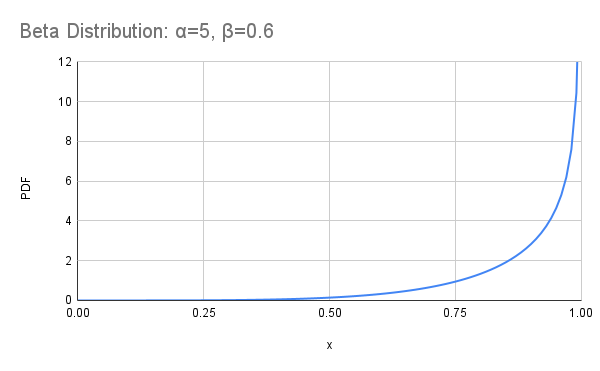
\includegraphics[scale=0.35]{media/beta.png}\end{center}
    \caption{Beta Distribution used in $\alpha\beta$-AWA*}\label{fig:beta}
\end{figure}

\section{Evaluation}
In order to evaluate the usefulness of exploration in AWA$^*$ a number of experiments were conducted on the sliding tile puzzle. All experiments are run on an 8-core 1.70GHz machine with 16 gigabytes of memory. For all experiments, the two exploration techniques will be compared to a standard AWA$^*$ implementation which will serve as the benchmark. One hundred instances of the unit cost 12-puzzle were used to compare the three algorithms.

The primary focus was on the Unit Cost Sliding Tile puzzle using the Manhattan Distance Heuristic. Various weights are used across the three algorithms and two different values of $\epsilon$, $0.1$ and $0.3$ \cite{valenzano2014comparison}, are used for $\epsilon-$AWA$^*$ and $\alpha \beta-$AWA$^*$. Depending on the value of $\epsilon$, $\epsilon-$AWA$^*$ and $\alpha \beta-$AWA$^*$ will be abbreviated to $0.1$-$\epsilon$, $0.3$-$\epsilon$, $0.1$-$\alpha \beta$, and $0.3$-$\alpha \beta$ respectively. The beta distribution in all $\alpha \beta-$AWA$^*$ instances is fixed at $\alpha=5$ and $\beta=0.6$.

There are also two small extensions. In the first, the Inverse Sliding Tile Puzzle is briefly investigated using the Manhattan Distance Heuristic. In these experiments, the value of $\epsilon$ is fixed at 0.3, and only 3 weights are considered: 1.3, 5, and 10. The Inverse Sliding Tile Puzzle was chosen because it tends to be harder than the Unit Cost variant. The second extension involves degrading the heuristic and using the Correct Tile Placement Heuristic. This was done to investigate how exploration may help or hinder with a highly uninformed heuristic.

\subsection{Unit Cost Tile Puzzle}
In general, it was found that adding exploration to AWA* for the sliding tile puzzle proved to be very effective. Both $\epsilon-$AWA$^*$ and $\alpha \beta-$AWA$^*$ required fewer incumbent solutions to zero in on the optimal solution, as summarized in Table \ref{tad:num-sol}.

\begin{table}
\def\arraystretch{1.3}
\begin{tabular}{ |c||c|c|c|c|c|  }
    \hline
    \multicolumn{6}{|c|}{Average Number of Incumbent Solutions} \\
    \hline
    Weight& AWA* & $0.1$-$\epsilon$ &$0.3$-$\epsilon$&$0.1$-$\alpha \beta$ & $0.3$-$\alpha \beta$\\
    \hline
    1.3 & \textbf{2.24} & 2.25 & 2.28 & 2.26 & 2.28\\
    \hline
    2 & 3.91 & 4.09 & \textbf{3.75} & 3.94 & 3.86\\
    \hline
    3 & 7.07 & 6.69 & \textbf{6.07} & 6.54 & 6.19\\
    \hline
    5 & 11.15 & 10.37 & \textbf{9.28} & 10.05 & 9.65\\
    \hline
    10& 15.49 & 15.03 & \textbf{13.27} & 14.56 & 13.74\\
    \hline
\end{tabular}
\caption{Incumbent Solutions}\label{tad:num-sol}
\end{table}

In all cases, except for weight=1.3, $0.1$-$\epsilon-$AWA$^*$ required the fewest incumbent solutions before finding the optimal. However, both exploration were consistently better than standard AWA* by this metric. 

To gauge the complexity of each algorithm the number expanded nodes and the total number of generated nodes are considered. By this metric exploration shows a huge improvement over standard AWA*, as shown in Figure \ref{fig:nodes}.

\begin{figure}
    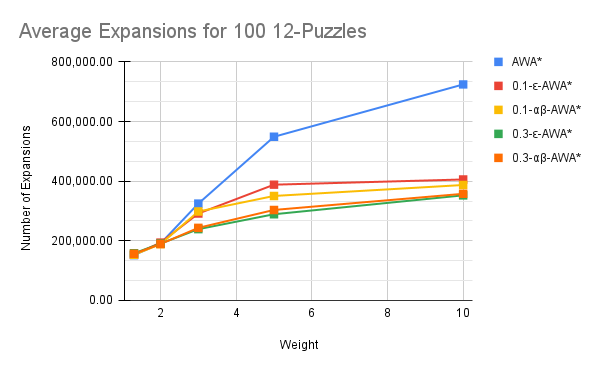
\includegraphics[width=\linewidth]{media/Average Expansions for 100 12-Puzzles.png}
    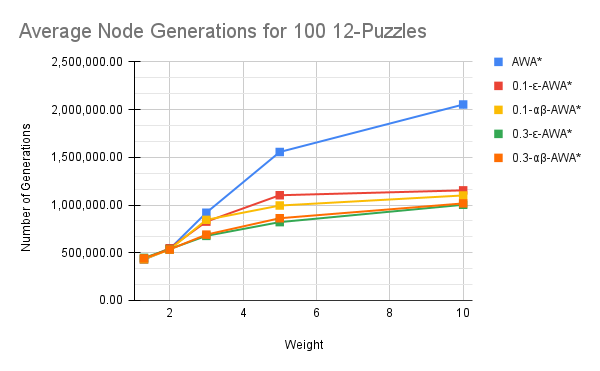
\includegraphics[width=\linewidth]{media/Average Node Generations for 100 12-Puzzles.png}
    \caption{Complexity with Manhattan Distance Heuristic.} \label{fig:nodes}
\end{figure}

Standard AWA* requires close to 800,000 expansions in the case of a weight of 10, while all four exploration algorithms require in the neighbourhood of 400,000. AWA* seems to be far more impacted by increasing the weight, and thereby degrading the accuracy of the evaluation function, than the $\epsilon$ and $\alpha\beta$ variants--which both require a similar number of expansions for a weight of 5 and a weight of 10. Perhaps most surprising is that setting $\epsilon$ to 0.3 gets the best results.

Adding to this, exploration in anytime sees an analogous improvement in its runtime when compared to standard AWA*, as seen in Figure \ref{fig:run}. This is not guaranteed as it could be the case that the improved node selection procedure takes enough time so as to offset the time savings of expanding fewer nodes. In the cases of $\epsilon-$AWA$^*$ and $\alpha \beta-$AWA$^*$, the node selection procedure is sufficiently simple that the expansion savings result in (proportionally) equal time savings. 

\begin{figure}
    \begin{center}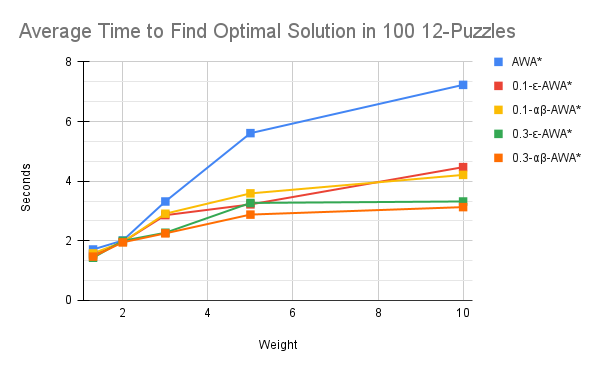
\includegraphics[scale=0.35]{media/Average Time to Find Optimal Solution in 100 12-Puzzles.png}\end{center}
    \caption{Average Time to Find Optimal Solution}\label{fig:run}
\end{figure}

To summarize the above results, it's useful to look at how quickly each algorithm converges on the optimal solution over time and over number of expansions. Given both the $\epsilon$ and $\alpha\beta$ variants required fewer incumbent solutions, fewer expansions to get those solutions, and took less time, it should be the case that they approach the optimal solution much faster than AWA*, which is precisely what we see in Figure \ref{fig:conv-man}.

\begin{figure}
    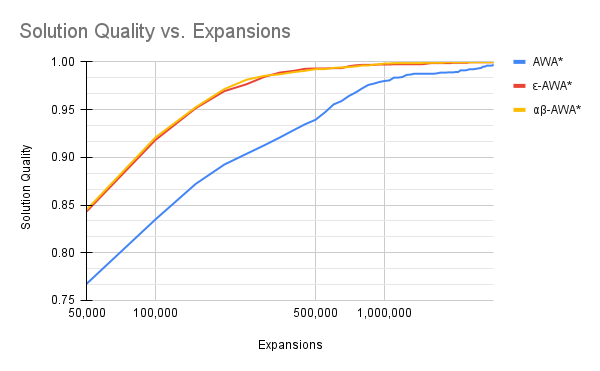
\includegraphics[width=\linewidth]{media/man-Solution Quality vs. Expansions.png}
    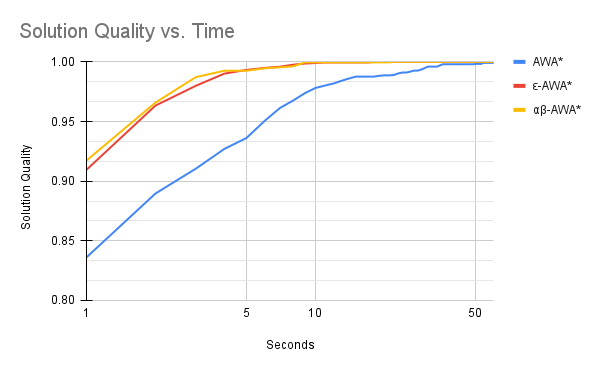
\includegraphics[width=\linewidth]{media/man-Solution Quality vs. Time.png}
    \caption{Quality Convergence with Manhattan Distance Heuristic.} \label{fig:conv-man}
\end{figure}

Here, solution quality is $\frac{incumbent-cost}{optimal-cost}$ for a given problem and the solution qualities are averaged across all problem instances. For expansion convergence, the incumbent cost was polled every 50,000 expansions; for the time convergence the incumbent cost was polled every one second (notice the log x-axis in both charts). In this, only a weight of 10 and an epsilon value of 0.3 were considered. 

\subsection{Inverse Cost Tile Puzzle}

\begin{table}
\def\arraystretch{1.3}
\begin{tabular}{ |c||c|c|c|  }
    \hline
    \multicolumn{4}{|c|}{Average Number of Incumbent Solutions} \\
    \hline
    Weight& AWA* & $0.3$-$\epsilon$-AWA$^*$ & $0.3$-$\alpha\beta$-AWA$^*$\\
    \hline
    1.3 & 3.14 & 3.13 & \textbf{2.97} \\
    \hline
    5 & 21.91 & 15.66 & \textbf{15.41} \\
    \hline
    10& 30.8 & \textbf{20.4} & 21.26 \\
    \hline
\end{tabular}
\caption{Incumbent Solutions}\label{tab:inv-sol}
\end{table}

\begin{table}
\def\arraystretch{1.3}
\begin{tabular}{ |c||c|c|c|  }
    \hline
    \multicolumn{4}{|c|}{Average Number of Seconds to Find Optimal} \\
    \hline
    Weight& AWA* & $0.3$-$\epsilon$-AWA$^*$ & $0.3$-$\alpha\beta$-AWA$^*$\\
    \hline
    1.3 & 2.25 & \textbf{2.15} & \textbf{2.15} \\
    \hline
    5 & 16.38 & 6.65 & \textbf{6.34} \\
    \hline
    10& 21.57 & \textbf{7.3} & 8.09 \\
    \hline
\end{tabular}
\caption{Runtime}\label{tab:inv-avg-time}
\end{table}

\begin{table}
\def\arraystretch{1.3}
\begin{tabular}{ |c||c|c|c|  }
    \hline
    \multicolumn{4}{|c|}{Average Number of Expansions} \\
    \hline
    Weight& AWA* & $0.3$-$\epsilon$-AWA$^*$ & $0.3$-$\alpha\beta$-AWA$^*$\\
    \hline
    1.3 & \textbf{186,038.15} & 211,198.92 & 206,175.07 \\
    \hline
    5 & 1,408,646.74 & 622,837.79 & \textbf{587,692.64} \\
    \hline
    10& 1,901,236.58 & \textbf{709,049.28} & 769,546.95 \\
    \hline
\end{tabular}
\caption{Expansions}\label{tab:inv-avg-exp}
\end{table}

\begin{table}
\def\arraystretch{1.3}
\begin{tabular}{ |c||c|c|c|  }
    \hline
    \multicolumn{4}{|c|}{Average Number of Node Generations} \\
    \hline
    Weight& AWA* & $0.3$-$\epsilon$-AWA$^*$ & $0.3$-$\alpha\beta$-AWA$^*$\\
    \hline
    1.3 & \textbf{529,095.35} & 603,706.60 & 589,437.60 \\
    \hline
    5 & 4,003,219.50 & 1,780,788.61 & \textbf{1,680,521.61} \\
    \hline
    10& 5,401,559.63 & \textbf{2,027,138.81} & 2,200,575.94 \\
    \hline
\end{tabular}
\caption{Generations}\label{tab:inv-avg-gen}
\end{table}

\subsection{Degraded Heuristic in Unit Cost Sliding Tiles}
Given the promising results above, it would be expected that when the heuristic gets degraded, exploration should help even more as degraded heuristics result in more plateaus and less confidence about the `best' node in the open list. However, in looking at the summary evaluation of solution quality over time and expansions using the Correct Tile Placement heuristic, this did not turn out to be case, as seen in Figure \ref{fig:conv-correct}.

Here, again, only a weight of 10 and an epsilon value of 0.3 were considered. For expansions, each algorithm was limited to 3,000,000 expansions, and for time each algorithm was limited to one minute. 

\begin{figure}
    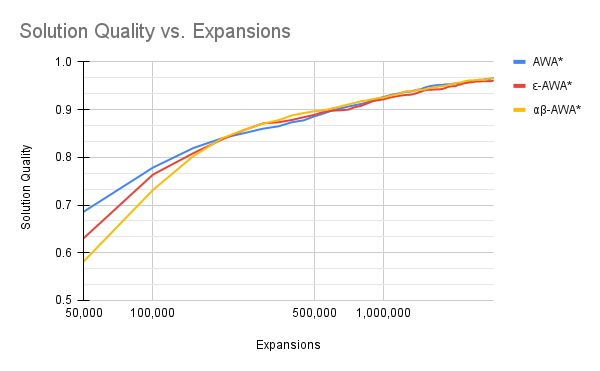
\includegraphics[width=\linewidth]{media/correct-Solution Quality vs. Expansions.png}
    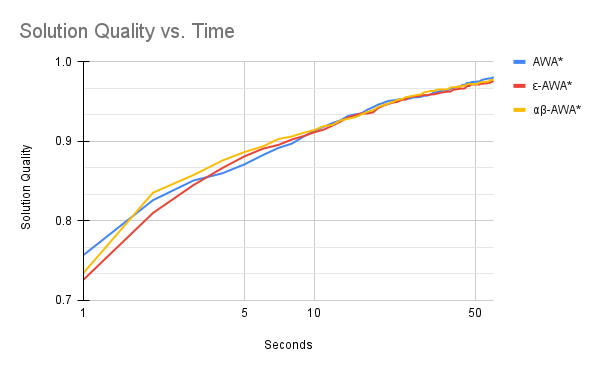
\includegraphics[width=\linewidth]{media/correct-Solution Quality vs. Time.png}
    \caption{Quality Convergence with Correct Tile Placement Heuristic.} \label{fig:conv-correct}
\end{figure}

While in the beginning AWA* actually has the best incumbent solutions, they all more or less approach the optimal solution at the same rate. This seems to simply demonstrate just how bad the Correct Placement heuristic is. I think what is going on here is that the Correct Placement heuristic is so bad it affectively adds and pulls nodes from the open list at random and so adding an exploration technique in no way helps since choosing the `best' node is also, basically, exploratory.

% \begin{figure*}
% 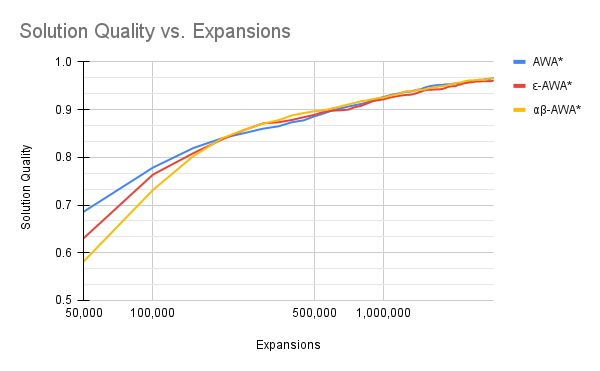
\includegraphics{media/correct-Solution Quality vs. Expansions.png}
% 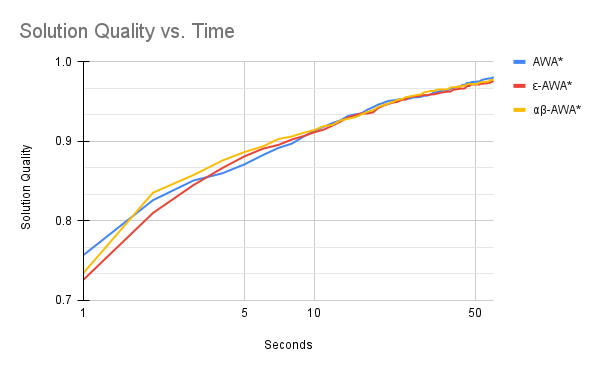
\includegraphics{media/correct-Solution Quality vs. Time.png}
% \caption{Quality Convergence with a Bad Heuristic.} \label{fig:conv-correct}
% \end{figure*}



\section{Discussion and Conclusion}
While the results above are promising, the experimentation done was very limited in its scope and left a lot to be desired. 

For starters, very few domains were investigated. Just investigating the tile puzzle makes it difficult to make any general statements about these results. 

The investigation into $\alpha \beta$-AWA$^*$ was incomplete because the beta distribution was fixed for all experiments. Discovering any merits or shortcomings of $\alpha \beta$-AWA$^*$ would require a whole set of experiments examining different distributions across various domains. Based on these early results I'd say $\alpha \beta$-AWA$^*$ looks interesting, but the fact it was not convincingly better than random sampling means more experimentation needs to be done. 

There are many other exploration techniques that could be evaluated in an anytime context. Type-Based exploration, which appears to perform very well in many domains would be an obvious starting point. 

Lastly, the results of exploration in the Inverse Cost Tile Puzzle were very surprising and definitely worth a closer look.  

Ultimately, I think this was a useful pilot study into using randomized exploration in an anytime search algorithm, but still more investigation is required before anything definitive is said.




\newpage
\bibliography{ref}
% \bibliographystyle{aaai22}

\end{document}